\documentclass[conference]{IEEEtran}
\IEEEoverridecommandlockouts
% The preceding line is only needed to identify funding in the first footnote. If that is unneeded, please comment it out.
\usepackage{cite}
\usepackage{amsmath,amssymb,amsfonts}
\usepackage{algorithmic}
\usepackage{graphicx}
\usepackage{textcomp}
\usepackage{xcolor}
\def\BibTeX{{\rm B\kern-.05em{\sc i\kern-.025em b}\kern-.08em
    T\kern-.1667em\lower.7ex\hbox{E}\kern-.125emX}}
\begin{document}

\title{NETWORK INTRUSION DETECTION USING MACHINE LEARNING: AN OVERVIEW}

\author{\IEEEauthorblockN{Gbenga S. Agunsoye}
\IEEEauthorblockA{\textit{Department of Computer Science} \\
\textit{Prairie View A\&M University}\\
Prairie View, United States. \\
gagunsoye@student.pvamu.edu}}

\maketitle

\begin{abstract}
As attackers continually device means to obfuscate attacks, the need for rapid measures to constantly detect vulnerabilities and mitigate threats within Networks arises. A variety of approaches used in developing systems that capture data packets travelling on the network media in order to ascertain their verity exist, including Anomaly-based techniques, signature based techniques or both. One issue remains constant in determining the efficacy of any of this approach – that is, the quality of data-set. In this paper, we review previous work that has been done using similar approach
\end{abstract}

\begin{IEEEkeywords}
IDS, Attack, DDoS, Artificial Intelligence, Machine Learning, Deep Learning
\end{IEEEkeywords}

\section{Introduction}
Machine Learning and artificial intelligence has become an invaluable approach to understanding the behaviour of network traffic in order to distinguish between benign and abnormal traffic. Hence, modern day intrusion detection system heavily employ this technique to adequately classify network traffic, consequently, improving the accuracy of detection of attacks such as Heartbleed, DoS Hulk, DoS GoldenEye, Bot, PortScan and Web Attack.
A Network attack is a deliberate infiltration of a Network by an attacker. It is a deliberate disruption of the normal flow of events that facilitates end to end connectivity of devices in a Network. Thereby, hampering the exchange of information from between two or more entities or devices.
Intrusion Detection is a set of techniques and methods that are used to detect suspicious activity both at the network and host level. Its role of forewarning administrators about intrusions, attacks or malware behavior cannot be overemphasized. Iman Sharafaldin et al. emphasized that having an IDS is mandatory in order to keep a strong line of defense for protecting critical networks against these ever increasing issues of intrusive activities. There are two dominant methods of finding exploits within a network traffic, which are Signature-based Intrusion Detection (SID) and Anomaly-based Intrusion Detection (AID). Anomaly-based IDS are trained to continuously observed normal patterns of behavior and recognize any deviation, while Signature-based IDS compare signature of attacks with those in existing records. A plethora of research has been undertaken to undermine the strengths of each of these methods as well as loopholes that exist in each of them and are being exploited by attackers. Sections II to V outlines related works and results achieved, while section VI clearly defines the focus of this research. 


\section{Toward Generating a New Intrusion Detection Dataset and Intrusion Traffic Characterization}

\subsection{Maintaining the Integrity of the Specifications}

Iman Sharafaldin et al.\cite{sharalfaldin2018} in their work, used CICFlowMeter to generate and extracted 80 traffic features from their dataset. They employed different classifiers including KNN, RF, ID3, Adaboost, MLP, Naïve-Bayes, and QDA. The performance report of their work showed varying results for Precision (Pr), Recall (Rc), F-Measure (F1), as well as execution time (in secs), which is given below.
\begin{table}[bt]
\caption{The Performance Examination Results}
    \begin{center}
    \begin{tabular}{|l|c|c|c|c|} \hline
    \textbf{Algorithm} & \textbf{Pr}
    & \textbf{Rc} & \textbf{F1} & \textbf{Execution(Sec.)} \\ \hline
    {KNN} & {0.96} & {0.96} & {0.96} & {1908.23}\\
    {RF} & {0.98} & {0.97} & {0.97} & {74.39}\\
    {ID3} & {0.98} & {0.98} & {0.98} & {235.02}\\
    {Adaboost} & {0.77} & {0.84} & {0.77} & {1126.24}\\
    {MLP} & {0.77} & {0.83} & {0.76} & {575.73}\\
    {Naive-Bayes} & {0.88} & {0.04} & {0.04} & {14.77}\\
    {QDA} & {0.97} & {0.88} & {0.92} & {18.79}\\
    \hline
    \end{tabular}
    \end{center}
\end{table}
    
    
\section{Detecting Distributed Denial of Service Attacks Using Data Mining Techniques}
In their work, Alkasassbeh et al. incorporated three well-known classification techniques, which includes: Multilayer Perceptron (MLP), Naive Bayes and Random Forest \cite{Alkasassbeh2016}. They explained how they used Data mining techniques to detect Distributed Denial of Service (DDoS) Attacks. The steps involved collection and auditing, preprocessing file format, feature extraction and statistical measurement. The Transfer function employed was Sigmoid. The Sigmoid activation function is given in \eqref{eq1}
\begin{equation}
Z(x) = \frac{1}{1+e^\textsuperscript{-x}\label{eq1}}
\end{equation}
Their result after applying the three machine learning algorithms on the collected dataset classified the attacks into DDoS attacks into UDP Flood, Smurf, SIDDoS, HTTPFlood. They claimed that MLP classifier achieved the highest accuracy.

\section{A Convolutional Neural Network for Network Intrusion Detection System}
Leila et al carried out an extensive work on Intrusion Detection System using Convolutional Neural Network. CNN-NID is a deep learning method that enables NIDS to detect the class of normal and abnormal data \cite{Mohammadpour2018}.
They introduced the basic concepts of anomaly-based NIDS, deep learning techniques and NSL-KDD dataset. Their model was implemented using Python and Keras on a machine equipped with 16GB RAM and CPU Intel Core i7 installed with Windows 10. They claimed that the extracted features in the convolutional layers are robust to noises.

\section{Survey of intrusion detection systems:
techniques, datasets and challenges}
     Ansam Khraisat et al., carried out a survey of IDS and outlined the challenges of each technique employed.\cite{Khraisat2019}. Their work focused on:
     \begin{itemize}
         \item Classifying various kinds of IDS with the major types of attacks based on intrusion methods.
        \item Presenting a classification of network anomaly IDS evaluation metrics and discussion on the importance of the feature selection.
        \item Evaluation of available IDS datasets discussing the
challenges of evasion techniques
     \end{itemize}
     \subsection{Signature-based intrusion detection systems (SIDS)}
     Signature intrusion detection systems (SIDS) are based on pattern matching techniques to find a known attack; these are also known as Knowledge-based Detection or Misuse Detection \cite{Khraisat2019}.
     \subsection{Anomaly-based intrusion detection system (AIDS)}
     IDS has drawn interest from a lot of scholars due to its capacity to overcome the limitation of SIDS. In AIDS, a normal model of the behavior of a computer system is created using machine learning, statistical-based or knowledge-based methods. Any significant deviation between the observed behavior and the model is regarded as an anomaly, which can be interpreted as an intrusion \cite{Khraisat2019}. The assumption for this group of techniques is that malicious behavior differs from typical user behavior. The behaviors of abnormal users which are dissimilar to standard behaviors are classified as intrusions. Development of AIDS comprises two phases: the training phase and the testing phase. In the training phase, the normal traffic profile is used to learn a model of normal behavior, and then in the testing phase, a new data set is used to establish the system’s capacity to generalise to previously unseen intrusions. AIDS can be classified into a number of categories based on the method used for training, for instance, statistical based, knowledge-based and machine learning based (Butun et al., 2014). The main advantage of AIDS is the ability to identify zero-day attacks due to the fact that recognizing the abnormal user activity does not rely on a signature database (Alazab et al., 2012).\ref{fig:ML_Algorithm} shows the conceptual working of AIDS approach based on machine learning \cite{Khraisat2019}
     
         \begin{figure}[htbp]
    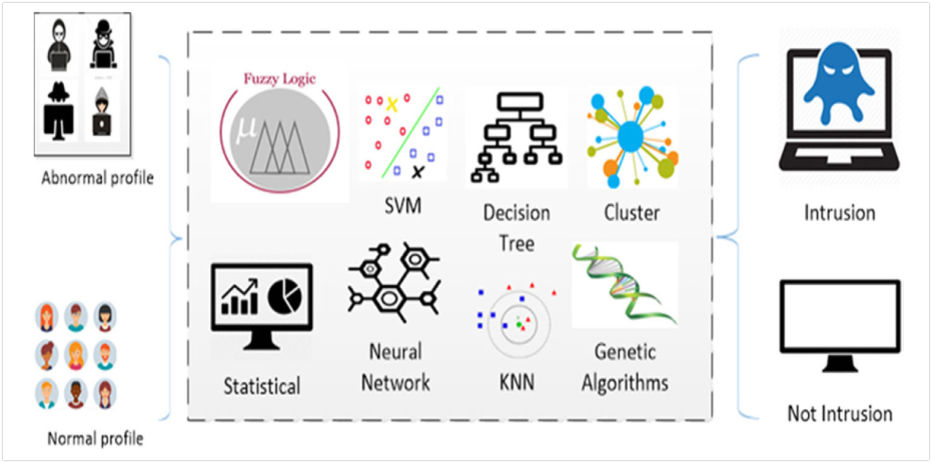
\includegraphics[scale=0.35]{ML_Algorithm.png}
    \caption{Conceptual working of AIDS approaches based on machine learning}
    \label{fig1}
    \end{figure}

\section{A Deep Learning Approach for Network Intrusion Detection System}
    In their work, Niyaz et al. gave an overview of Self-taught learning and NSL-KDD Dataset. Self-taught Learning (STL) is a deep learning approach that consists of two stages for the classification. First, a good feature representation is learnt from a large collection of unlabeled data, xu, termed as Unsupervised Feature Learning (UFL). In the second stage, this learnt representation is applied to labeled data, xl, and used for the classification task. Although the unlabeled and labeled data may come from different distributions, there must be relevance among them \cite{Niyaz2016}.

\section{Research Focus}
    This research is aimed at using machine learning algorithms to identify and classify network attacks based on extracted features from network traffic. The goal is to develop a model that would classify raw network traffic data into various attack categories using similar approach and tune the data to achieve a more accurate result. Here, our focus is using a traffic generator CF20 from Spirent. We hope achieve better performance as this data is generated live and not simulated.
    We start by designing a network of computers, switches, routers and firewalls. Then, we subject the design to attack traffic using the Spirent Cyberflood CF20 traffic generator. We then mirror our port to capture traffic data to observe the behaviour of our test device to these traffic. Then we develop a machine learning model that would classify our traffic into various attack categories based on some extracted features from the dataset.
    
\section*{Acknowledgment}

    I want to say a big thank you to Dr. Lin Li, associate professor, department of Computer Science, Prairie View A\&M University, for his supervision of this work and introducing the concept of professional writing using \LaTeX.


\bibliographystyle{plain}
\bibliography{references}

\end{document}
